\documentclass[letterpaper]{article}
\usepackage[margin=1in]{geometry}
\usepackage[utf8]{inputenc}
\usepackage{textcomp}
\usepackage{amssymb}
\usepackage{natbib}
\usepackage{graphicx}
\usepackage{gensymb}
\usepackage{amsthm, amsmath, mathtools}
\usepackage[dvipsnames]{xcolor}
\usepackage{enumerate}
\usepackage{mdframed}
\usepackage[most]{tcolorbox}
\usepackage{csquotes}
% https://tex.stackexchange.com/questions/13506/how-to-continue-the-framed-text-box-on-multiple-pages

\tcbuselibrary{theorems}

\newcommand{\R}{\mathbb{R}}
\newcommand{\Z}{\mathbb{Z}}
\newcommand{\N}{\mathbb{N}}
\newcommand{\Q}{\mathbb{Q}}
\newcommand{\C}{\mathbb{C}}
\newcommand{\code}[1]{\texttt{#1}}
\newcommand{\mdiamond}{$\diamondsuit$}
\newcommand{\PowerSet}{\mathcal{P}}
\newcommand{\Mod}[1]{\ (\mathrm{mod}\ #1)}
\DeclareMathOperator{\lcm}{lcm}

%\newtheorem*{theorem}{Theorem}
%\newtheorem*{definition}{Definition}
%\newtheorem*{corollary}{Corollary}
%\newtheorem*{lemma}{Lemma}
\newtheorem*{proposition}{Proposition}


\newtcbtheorem[number within=section]{theorem}{Theorem}
{colback=green!5,colframe=green!35!black,fonttitle=\bfseries}{th}

\newtcbtheorem[number within=section]{definition}{Definition}
{colback=blue!5,colframe=blue!35!black,fonttitle=\bfseries}{def}

\newtcbtheorem[number within=section]{corollary}{Corollary}
{colback=yellow!5,colframe=yellow!35!black,fonttitle=\bfseries}{cor}

\newtcbtheorem[number within=section]{lemma}{Lemma}
{colback=red!5,colframe=red!35!black,fonttitle=\bfseries}{lem}

\newtcbtheorem[number within=section]{example}{Example}
{colback=white!5,colframe=white!35!black,fonttitle=\bfseries}{def}

\newtcbtheorem[number within=section]{note}{Important Note}{
        enhanced,
        sharp corners,
        attach boxed title to top left={
            xshift=-1mm,
            yshift=-5mm,
            yshifttext=-1mm
        },
        top=1.5em,
        colback=white,
        colframe=black,
        fonttitle=\bfseries,
        boxed title style={
            sharp corners,
            size=small,
            colback=red!75!black,
            colframe=red!75!black,
        } 
    }{impnote}
\usepackage[utf8]{inputenc}
\usepackage[english]{babel}
\usepackage{fancyhdr}
\usepackage[hidelinks]{hyperref}

\pagestyle{fancy}
\fancyhf{}
\rhead{CSE 101}
\chead{Friday, January 14, 2022}
\lhead{Lecture 6}
\rfoot{\thepage}

\setlength{\parindent}{0pt}

\begin{document}

\section{Strongly Connected Components}
The issue with our algorithm is that we recompute the postorder for every SCC we need to find. However, we don't need to do this; rather, after removing some strongly connected components to get $G'$, the largest postorder number of vertices in $G'$ is still in a sink component of $G'$. 

\subsection{Better Algorithm}
\begin{verbatim}
    SCCs(G)
        Run DFS(G^R), record postorders
        Mark all vertices as unvisited 
        For v in V in reverse postorder 
            If v not in a component yet     // if v is not visited 
                explore(v) on G-components found,
                marking new component 
\end{verbatim}

So, really, this is just 2 DFSs, so the runtime is $O(|V| + |E|)$. 

\section{Paths in Graphs}
DFS and \code{explore} allow us to determine \emph{if} it is possible to get from one vertex to another, and using the DFS tree, you can also find a path. However, this is often not an efficient path. This is because DFS picks one path and tries to go to the end of that path before trying a different path. If that path happens to be a not-so-ideal path, then we've taken a much longer path than necessary. For example, consider the following graph:
\begin{center}
    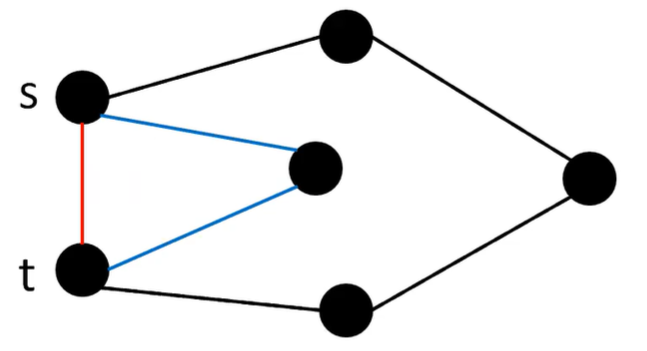
\includegraphics[scale=0.4]{../assets/dfs_bfs_comp.png}
\end{center}
Suppose we wanted to get from $s$ to $t$. Using DFS, we might take the black path; the one with 4 edges. How do we guarantee that we take the shortest path, i.e. the red path? 

\subsection{Goal}
Given a graph $G$ with two vertices $s$ and $t$ in the same connected component, how do we find the \emph{best} path from $s$ to $t$? In fact, what do we mean by the best path? 
\begin{itemize}
    \item Least expensive. 
    \item Best scenery.
    \item Shortest.
\end{itemize}
For now, we want the fewest edges. 

\subsection{Observation}
\begin{proposition}
    If there is a path from vertices $s$ to $v$ with length at most $d$, then there is some $w$ adjacent to $v$ where there is a path a length at most $(d - 1)$ from vertices $s$ to $w$.
\end{proposition} 

\begin{mdframed}[]
    \begin{proof}
        If $w$ is the next-to-last vertex on the path, then there are $d$ edges to get you from $s$ to $v$ and that means the number of edges you have to take from $s$ to $w$ is only $d - 1$. This means that if we know all of the vertices with distance at most $d - 1$, then we can find all of the vertices with distance at most $d$.
    \end{proof}
\end{mdframed}

For example, consider the following (annotated) graph:
\begin{center}
    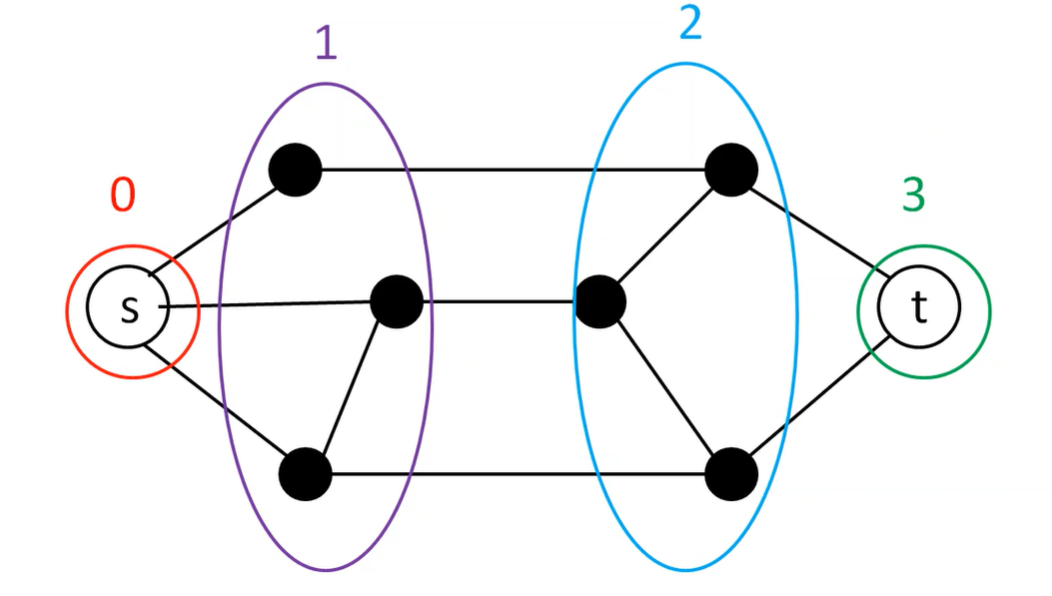
\includegraphics[scale=0.4]{../assets/1_2_3_dist.png}
\end{center}
Here, suppose we start at $s$.
\begin{itemize}
    \item The only place we can get with a path of length 0 is $s$, or the one vertex in the red circle labeled \code{0}.
    \item If we want to travel one edge, the only places we can get with a path of length one are the vertices in the purple circle labeled \code{1}.
    \item If we want to travel two edges, we can get to some vertex that is adjacent to one of the vertices in the purple circle. For each of the purple vertices, if we list all of the adjacent vertices, the only new vertices we can reach are the vertices in the cyan circle labeled \code{2}.
    \item Finally, if we want to travel three edges, we can get to something that is adjacent to the vertices at distance 2, which means we can get to $t$, or the vertex in the green circle labeled \code{3}. 
\end{itemize}
By the way we constructed these sets (the circles), it's not possible to get to $t$ at distance 2 because, for that to happen, it has to be adjacent to the vertices at distance 1, which it isn't.

\subsection{Algorithm Idea}
This observation gives us a pretty reasonable way to find an algorithm. In particular, if we want to find the best path length between $s$ and $t$, we really need to find the best path length between $s$ and every other vertex in the graph.

\bigskip 

So, the idea is, for each $d$, create a list of all vertices at distance $d$ from $s$.
\begin{itemize}
    \item For $d = 0$, this is just $\{s\}$.
    \item For larger $d$, we want all new vertices adjacent to vertices at distance $d - 1$.
\end{itemize}

\subsubsection{Algorithm}
The algorithm is as follows:
\begin{verbatim}
    1    ShortestPaths(G, s)
    2        Initialize Array A
    3        A[0] = {s}
    4        dist(s) = 0
    5        For d = 0 to n
    6            For u in A[d]
    7                For (u, v) in E
    8                    if dist(v) undefined
    9                        dist(v) = d + 1
    10                       add v to A[d + 1]
\end{verbatim}

\subsubsection{Improving the Algorithm}
How can we improve this?
\begin{itemize}
    \item What if \code{dist(v)} undefined at end? We can set the distances of all vertices to infinity.\footnote{Note that \code{+} next to a line number means added code and \code{c} next to a line number means changed line.}
    \begin{verbatim}
        1    ShortestPaths(G, s)
        2+       For each v in V, dist(v) = infinity 
        3        Initialize Array A
        4        A[0] = {s}
        5        dist(s) = 0
        6        For d = 0 to n
        7            For u in A[d]
        8                For (u, v) in E
        9c                   if dist(v) = infinity
        10                       dist(v) = d + 1
        11                       add v to A[d + 1]
    \end{verbatim}
    Here, at the end of the algorithm, any vertices that could not be found will be assigned a distance of infinity to indicate that it could not be reached. 

    \item The algorithm goes through \code{A[0]}, \code{A[1]}, and so on in order. We can just use a queue.
    \begin{verbatim}
        1    ShortestPaths(G, s)
        2        For each v in V, dist(v) = infinity 
        3c       Initialize Queue Q
        5        dist(s) = 0
        6c       While Q not empty
        7c           u = front(Q)
        8            For (u, v) in E
        9                if dist(v) = infinity
        10c                  dist(v) = dist(u) + 1
        11c                  Q.enqueue(v)
    \end{verbatim}

    \item What if we want to keep track of the paths? 
    \begin{verbatim}
        1    ShortestPaths(G, s)
        2        For each v in V, dist(v) = infinity 
        3        Initialize Queue Q
        4        dist(s) = 0
        5        While Q not empty
        6            u = front(Q)
        7            For (u, v) in E
        8                if dist(v) = infinity
        9                    dist(v) = dist(u) + 1
        10                   Q.enqueue(v)
        11+                  v.prev = u     // Keep track of path
    \end{verbatim}
    With this change, we can simply follow the chain of \code{prev}ious vertices, which is the path that was taken. 
\end{itemize}

\subsection{Breadth First Search}
In our last change above, we note that we simply have BFS.
\begin{verbatim}
    BFS(G, s)
        For v in V, dist(v) = infinity 
        Initialize Queue Q
        Q.enqueue(s)
        dist(s) = 0
        While Q is not empty
            u = front(Q)
            For (u, v) in E
                If dist(v) = infinity
                    dist(v) = dist(u) + 1
                    Q.enqueue(v)
                    v.prev = u
\end{verbatim}
The total runtime is $O(|V| + |E|)$.
\begin{itemize}
    \item In the first few lines, we have $O(|V|)$ time.
    \item In the while loop and the \code{front(Q)} lines, we have $O(|V|)$ iterations. 
    \item In the edge iteration, we have $O(|E|)$ iterations. 
\end{itemize}

\subsection{DFS vs. BFS}
\begin{itemize}
    \item Similarities:
    \begin{itemize}
        \item The way both algorithms process vertices is the same (\code{visited} for DFS vs. \code{dist < infinity} for BFS).
        \item For each vertex, process all unprocessed neighbors.
    \end{itemize}
    \item Differences:
    \begin{itemize}
        \item DFS uses a stack to store vertices waiting to be processed. 
        \item BFS uses a queue.
    \end{itemize}
    \item Big Effect:
    \begin{itemize}
        \item DFS goes depth-first: very long path. Get a very ``skinny'' tree. 
        \item BFS is breadth first: visits all side paths. Get a very shallow tree since we process all of the neighbors.
    \end{itemize}
\end{itemize}

\subsubsection{Relevant XKCD}
\begin{center}
    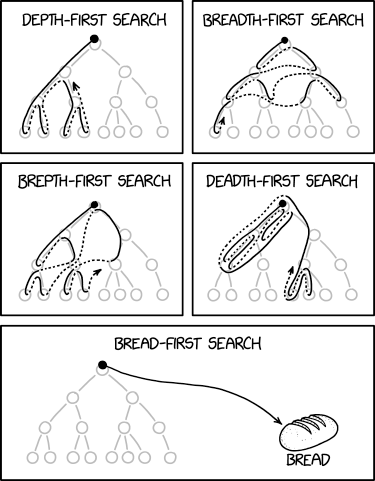
\includegraphics[scale=0.7]{../assets/xkcd_depth_and_breadth.png}
\end{center}

\subsection{Edge Length}
The number of edges in a path is not always the right measure of distance. Sometimes, taking several shorter steps is preferably to taking a few longer ones. 

\bigskip 

We can assign each edge $(u, v)$ a non-negative \underline{length} $\ell(u, v)$. The length of a path is the sum of the lengths of its edges.

\subsection{Problem: Shortest Path}
Coming soon!


\end{document}